Die wichtigsten Eigenschaften einer Beschreibungslogik sind
\emph{Ausdrucksstärke} und \emph{Komplexität}. Ausdrucksstärke kann man nicht
linear quantifizieren, sondern nur beschreiben und charakterisieren.

\subsection{Bisimulation}\label{bisimulation}

Die Bisimulation ist ein graphentheoretische Begriff, der die \enquote{Ähnlichkeit} von Graphen beschreibt und eng mit der Ausdrucksstärke von $\ALC$ zusammenhängt.

\begin{definition}[Bisimulation]

Seien $\MI_1$ und $\MI_2$ Interpretationen. Relation
$\rho \subseteq \Delta^{\MI_1} \times \Delta^{\MI_2}$ ist Bisimulation
zwischen $\MI_1$ und $\MI_2$, wenn gilt:

\begin{enumerate}
\def\labelenumi{\arabic{enumi}.}
\item
  Wenn $d_1\text{\ $\rho$}\text{\ d}_2$, dann gilt für alle
  Konzeptnamen A: $d_1 \in A^{\MI_1}$ gdw. $d_2 \in A^{\MI_2}$.
\item
  Wenn $d_1\text{\ $\rho$}\text{\ d}_2$ und
  $\left( d_1,d_1' \right) \in r^{\MI_1}$ für beliebigen
  Rollennamen $r$, dann gibt es ein $d_2' \in \Delta^{\MI_2}$
  mit ${d'}_1\text{\ $\rho$}{\ d'}_2$ und
  $\left( d_2,d_2' \right) \in r^{\MI_2}$.
\item
  Wenn $d_1\text{\ $\rho$}\text{\ d}_2$ und
  $\left( d_2,d_2' \right) \in r^{\MI_2}$ für beliebigen
  Rollennamen $r$, dann gibt es ein $d_1' \in \Delta^{\MI_1}$
  mit ${d'}_1\text{\ $\rho$}{\ d'}_2$ und
  $\left( d_1,d_1' \right) \in r^{\MI_1}$.
\end{enumerate}
\end{definition}

\begin{tafel}[Beispiel Bisimulation] \mbox{}\\
    \begin{enumerate}
        \item \mbox{}
            \begin{center}
                \begin{tikzpicture}
                    \begin{scope}[every node/.style={circle,draw,thick}]
                        \node (s0) at (0, 0) {};
                        \node (s1) at (3, 0) {};
                    \end{scope}
                    \begin{scope}[every node/.style={fill=white}]
                        \node (name) at (0, 1) {$\MI_1$};
                        \node (name) at (3, 1) {$\MI_2$};
                        \node [left = 0.3cm of s0] at (s0){$A, A', B$};
                        \node [right = 0.3cm of s4] at (s1){$A, A', B$};
                        \path[dotted] [-] (s0) edge node {$\rho$}(s1);
                    \end{scope}
                \end{tikzpicture}
            \end{center}
        \item \mbox{}
            \begin{center}
                \begin{tikzpicture}
                    \begin{scope}[every node/.style={circle,draw,thick}]
                        \node (s0) at (0, 0) {};
                        \node (s1) at (3, 0) {};
                        \node (s2) at (0, -2) {};
                        \node (s3) at (3, -2) {};
                    \end{scope}
                    \begin{scope}[every node/.style={fill=white}]
                        \node (name) at (0, 1) {$\MI_1$};
                        \node (name) at (3, 1) {$\MI_2$};
                        \path[dotted] [-] (s0) edge node {$\rho$}(s1);
                        \path[dotted] [-] (s2) edge node {$\rho$}(s3);
                        \path [->] (s0) edge node {$r$}(s2);
                        \path [->] (s1) edge node {$r$}(s3);
                    \end{scope}
                \end{tikzpicture}
            \end{center}
        
        \item \mbox{}
            \begin{center}
                \begin{tikzpicture}
                    \begin{scope}[every node/.style={circle,draw,thick}]
                        \node (s0) at (0, 0) {};
                        \node (s1) at (3, 0) {};
                        \node (s2) at (5, 0) {};
                        \node (s3) at (7, 0) {};
                    \end{scope}
                    \begin{scope}[every node/.style={fill=white}]
                        \node (name) at (0, 1) {$\MI_1$};
                        \node (name) at (3, 1) {$\MI_2$};
                        \node (s4) at (9, 0) {$\cdots$};
                        \path[dotted] [-] (s0) edge [bend right] node {$\rho$}(s1);
                        \path[dotted] [-] (s0) edge [bend right] node {$\rho$}(s2);
                        \path[dotted] [-] (s0) edge [bend right] node {$\rho$}(s3);
                        \path [->] (s0) edge [loop left] node {$r$}(s0);
                        \path [->] (s1) edge node {$r$}(s2);
                        \path [->] (s2) edge node {$r$}(s3);
                        \path [->] (s3) edge node {$r$}(s4);
                    \end{scope}
                \end{tikzpicture}
            \end{center}
\end{tafel}

Seien $\MI_1$ und $\MI_2$ Interpretationen,
$d_1 \in \Delta^{\MI_1}$, $d_2 \in \Delta^{\MI_2}$.
Dann schreiben wir
\[(\MI_1,d_1) \sim (\MI_2,d_2),\] wenn es eine Bisimulation $\rho$
zwischen $\MI_1$ und $\MI_2$ gibt mit $d_1\text{\ $\rho$}\text{\ d}_2$. (Wir sagen \enquote{$d_1$ ist \emph{bisimilar zu} $d_2$}).
Die leere Relation ist immer eine Bisimulation.

\begin{theorem}[Bisimulationstheorem]
    \label{thm:bisim}
Seien $\MI_1$, $\MI_2$ Interpretationen,
$d_1 \in \Delta^{\MI_1}$ und $d_2 \in \Delta^{\MI_2}$. Wenn
$(\MI_1,d_1) \sim (\MI_2,d_2)$, dann gilt für alle $\ALC$-Konzepte
$C$:
\[d_1 \in C^{\MI_1} \gdw d_2 \in C^{\MI_2}\]
\end{theorem}

\begin{tafel}[Beweis des Bismulationstheorems] Beweis von \autoref{thm:bisim}
\begin{proof}
Beweisskizze per Induktion über die Struktur von $C$. Sei $\rho$ eine
Bisimulation zwischen $\MI_1$ und $\MI_2$ mit
$d_1\text{\ $\rho$}\text{\ d}_2$.

\textbf{I.A.} $C = A$ ist Konzeptname. Nach Bedingung 1. der
Bisimulation gilt
\[ d_1 \in A^{\MI_1} \gdw d_2 \in A^{\MI_2}. \]


\textbf{I.S.} Unterscheide Fälle gemäß des äußersten Konstruktes von C.
Es genügen $\neg$,$\sqcap$, $\exists\text{r.C}$:

\begin{enumerate}
\item $C = \neg D$
    \begin{align*}
        d_1 \in C^{\MI_1}
        &\gdw d_1 \notin D^{\MI_1} & \text{(Semantik)}\\
        &\gdw d_2 \notin D^{\MI_2} & \text{(I.V.)}\\
        &\gdw d_2 \in C^{\MI_2} & \text{(Semantik)}
    \end{align*}
\item $C = D_1 \sqcap D_2$
  \begin{align*}
d_1 \in C^{\MI_1}
&\gdw d_1 \in D_1^{\MI_1}\ und\ d_1 \in D_2^{\MI_1} & \text{(Semantik)}\\
&\gdw d_2 \in D_1^{\MI_2}\ und\ d_2 \in D_2^{\MI_2} & \text{(I.V.)}\\
&\gdw d_2 \in C^{\MI_2} & \text{(Semantik)}
\end{align*}

\item $C = \exists r.D$
  \begin{align*}
d_1 \in C^{\MI_1}
&\implies \exists e_1 : (d_1,e_1) \in r^{\MI_1}\ und\ e \in D^{\MI_1} & \text{(Semantik)}\\
&\implies \exists e_2 \in \Delta_2^{\MI_2}: (d_2,e_e) \in r^{\MI_2}\ und\ (e_1 \rho e_2) & \text{(2. Bedingung)}\\
&\implies e_2 \in D^{\MI_2} & \text{(I.V.)}\\
&\implies d_2 \in (\exists r.D)^{\MI_2} & \text{(Semantik)}\\
&\gdw d_2 \in C^{\MI_2} & \text{(Semantik)}
\end{align*}
\end{enumerate}
Rückrichtung analog, nur mit der 3. Bedingung.
\end{proof}
\end{tafel}

Intuitiv gesprochen kann $\ALC$ nicht zwischen $d_1$ und $d_2$ \enquote{unterscheiden}.

\subsubsection{Ausdrucksstärke}\label{ausdrucksstuxe4rke}

\begin{definition}[Eigenschaft, Ausdrückbarkeit]

Eine \emph{Eigenschaft} $E$ ist eine Menge von Paaren $(\MI,d)$, wobei
$\MI$ eine Interpretation und $d \in \Delta^\MI$ ein Element in $\MI$ ist.
$E$ ist \emph{ausdrückbar in $\ALC$}, wenn es ein $\ALC$-Konzept $C$
gibt, so dass für alle $\MI$ und $d \in \Delta^\MI$ gilt: 
\[ \left( \MI,\ d \right) \in E \gdw d \in C^\MI \]
\end{definition}

Intuitionen:
\begin{itemize}
    \item $d \in \Delta^\MI$ hat die Eigenschaft $E$ gdw. $(\MI, d) \in E$.
    \item $E$ ist ausdrückbar, wenn es ein \emph{äquivalentes} $\ALC$-Konzept $C$ gibt.
\end{itemize}

\subsubsection{Verwendung von Bisimulation I}\label{theorem-3.4}

\begin{theorem}[Beschränkungen der Ausdrucksstärke von $\ALC$]
    \label{thm:beschraenkt}
In $\ALC$ sind nicht ausdrückbar: 
\begin{itemize}
\item das $\ALCI$-Konzept $\exists r^{-}.\top$ 
\item die $\ALCQ$-Konzepte
\begin{itemize}
  \item $\leq n\ r.\top$ für alle $n > 0$ und
  \item $\geq n\ r.\top$ für alle $n > 1$
\end{itemize}
\end{itemize}
\end{theorem}


\begin{tafel}[Beweisskizze] Finde Bisimulation für die dies nicht gilt.

\begin{proof} $\exists r^{-}.\top$ ist nicht $\ALC$-ausdrückbar.
 Betrachte zwei Interpretationen $\MI$ und $\MJ$

 \begin{center}
     \begin{tikzpicture}
         \begin{scope}[every node/.style={circle,draw,thick}]
             \node (s0) at (0, 0) {$d$};
             \node (s1) at (3, -2) {$x$};
             \node (s2) at (0, -2) {$e$};
         \end{scope}
         \begin{scope}[every node/.style={fill=white}]
             \node (name) at (0, 1) {$\MI$};
             \node (name) at (3, 1) {$\MJ$};
             \path[dotted] [-] (s2) edge node {$\rho$}(s1);
             \path [->] (s0) edge node {$r$}(s2);
         \end{scope}
     \end{tikzpicture}

     $(\MI, e) \sim (\MJ, x)$ bisimilar
 \end{center}

Angenommen, es gäbe ein $\ALC$-Konzept $C$ mit $C \equiv \exists r^{-}.\top$. Dann gilt $e \in C^\MI$. Mit \autoref{thm:bisim} folgt $x \in C^{\MJ}$, also hat $x$ auch einen $r$-Vorgänger in $\MJ$. $\lightning$
\end{proof} 

\begin{proof} $\leq n\ r.\top$ ist nicht $\ALC$-ausdrückbar.

Betrachte zwei Interpretationen $\MI$ und $\MJ$

 \begin{center}
     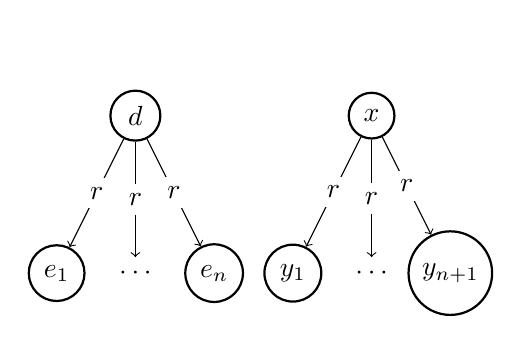
\begin{tikzpicture}
         \begin{scope}[every node/.style={circle,draw,thick}]
             \node (s0) at (0, 0) {$d$};
             \node (s2) at (-1, -2) {$e_1$};
             \node (s4) at (1, -2) {$e_n$};
             \node (s1) at (3, 0) {$x$};
             \node (s5) at (2, -2) {$y_1$};
             \node (s7) at (4, -2) {$y_{n + 1}$};
         \end{scope}
         \begin{scope}[every node/.style={fill=white}]
             \node (name) at (0, 1) {$\MI$};
             \node (name) at (3, 1) {$\MJ$};
             \node (s3) at (0, -2) {$\cdots$};
             \node (s6) at (3, -2) {$\cdots$};
             \path [->] (s0) edge node {$r$}(s2);
             \path [->] (s0) edge node {$r$}(s3);
             \path [->] (s0) edge node {$r$}(s4);
             \path [->] (s1) edge node {$r$}(s5);
             \path [->] (s1) edge node {$r$}(s6);
             \path [->] (s1) edge node {$r$}(s7);
         \end{scope}
     \end{tikzpicture}
 \end{center}
 Bisimulation
 \[
     \rho = \{ (d, x) \} \cup \{ (e_i, y_j) \mid i \leq n, j \leq n + 1 \}
 \]
 Angenommen, es gäbe ein $\ALC$-Konzept $C$ mit $C \equiv \leq n\ r.\top$. Dann gilt $d \in C^\MI$. Mit \autoref{thm:bisim} folgt $x \in C^{\MJ}$, also $x \in \leq n\ r.\top$. $\lightning$
\end{proof}
\end{tafel}

Man sieht, dass die Argumentation zum Beweis der Nicht-Ausdrückbarkeit immer auf dasselbe hinausläuft:

\begin{theorem}[$\ALC$ Nicht-Ausdrückbarkeit]
    \label{thm:alc-nicht-ausdruck}
Sei $E$ eine Eigenschaft. Wenn es Interpretation $\MI_1$, $\MI_2$
und Elemente $d_1 \in \Delta^{\MI_1}$ und
$d_2 \in \Delta^{\MI_2}$ gibt, so dass

\begin{itemize}
\item
  $\left( \MI_1,d_1 \right) \in E$ und
  $\left( \MI_2,d_2 \right) \not\in E$ sowie
\item
  $(\MI_1,d_1) \sim (\MI_2,d_2)$,
\end{itemize}

dann ist $E$ nicht in $\ALC$ ausdrückbar.
\end{theorem}

\subsubsection{Verwendung von Bisimulation II}

Eine Interpretation ist ein \emph{Baum} gdw. $(\Delta^\MI, \cdot^\MI)$
Baum (endlich oder unendlich). Konzept $C$ und TBox $\MT$ haben
\emph{gemeinsames Baummodell} $\MI$, wenn $\MI$ Modell von $\MT$ und Baum mit
Wurzel $d$ sowie $d \in C^\MI$.

$\ALC$ hat die \emph{Baummodelleigenschaft}.

\begin{theorem}[$\ALC$ Baummodelleigenschaft]
    \label{theorem-3.6}
    \label{thm:baummodell}
Wenn ein ALC-Konzept $C$ bezüglich einer ALC-TBox $\MT$ erfüllbar ist,
dann haben $C$ und $\MT$ ein \emph{gemeinsames Baummodell} $\MI$. (mit $\MI$ Baum, Wurzel in $C^\MI$.)
\end{theorem}

\begin{tafel}[Beispiel Baummodell]
    \begin{align*}
        C &= A \sqcap \exists s.B \sqcap \forall s.\exists r.A\\
        \MT &= \{ \top \sqsubseteq \exists s.A \}
    \end{align*}

 \begin{center}
     \begin{tikzpicture}
         \begin{scope}[every node/.style={circle,draw,thick}]
             \node (s0) at (0, 0) {};
             \node (s1) at (-1, -2) {};
             \node (s2) at (1, -2) {};
             \node (s3) at (-2, -4) {};
             \node (s4) at (0, -4) {};
             \node (s6) at (-2, -6) {};
         \end{scope}
         \begin{scope}[every node/.style={fill=white}]
             \node (s5) at (1, -3) {$\vdots$};
             \node (s7) at (0, -5) {$\vdots$};
             \node (s8) at (-2, -7) {$\vdots$};
             \node [right = 0.3cm of s0] at (s0){$A$};
             \node [right = 0.3cm of s2] at (s2){$A$};
             \node [right = 0.3cm of s4] at (s4){$A$};
             \node [right = 0.3cm of s6] at (s6){$A$};
             \node [left = 0.3cm of s1] at (s1){$B$};
             \node [left = 0.3cm of s3] at (s3){$A$};
             \path [->] (s0) edge node {$s$}(s2);
             \path [->] (s0) edge node {$s$}(s1);
             \path [->] (s1) edge node {$r$}(s3);
             \path [->] (s1) edge node {$s$}(s4);
             \path [->] (s3) edge node {$s$}(s6);
         \end{scope}
     \end{tikzpicture}
 \end{center}
\end{tafel}

Die Baummodelleigenschaft ist Grundlage für Algorithmen und erlaubt Aussagen über die Ausdrucksstärke.

\subsubsection{Unravelling}\label{unravelling}

Sei $\MI$ eine Interpretation und $d \in \Delta^\MI$. 
Dann ist ein $d$-Pfad in $\MI$ eine Sequenz $d_1\cdots d_n$, $n \geq 1$ mit $d_1 = d$ und
für alle $i < n$ gilt: es gibt einen Rollennamen $r$ mit $(d_i, d_{i + 1}) \in r^\MI$
\[\text{end}(d_1d_2\cdots d_n) = d_n\]

\begin{definition}[Unravelling]
Das Unravelling von $\MI$ an Stelle $d$ ist folgende Interpretation $\MJ$:
\begin{align*}
    \Delta^{\MJ} &= \text{Menge aller }d\text{-Pfade in }\MI\\
    A^{\MJ} &= \left\{ p \in \Delta^{\MJ}\  \right|\text{\ end}\left( p \right) \in A^\MI\}\\
    r^{\MJ} &= \left\{ \left( p,p' \right) \in \Delta^{\MJ} \times \Delta^{\MJ}\ |\ \exists e:p' = p \cdot e\ \mathrm{\text{und}}\ \left( \text{end}\left( p \right),e \right) \in r^\MI \right\}
\end{align*}
für alle Konzeptnamen $A$ und Rollennamen $r$
\end{definition}

\begin{tafel}[Beispiel Unravelling] \mbox{}
 \begin{center}
     \begin{tikzpicture}
         \begin{scope}[every node/.style={circle,draw,thick}]
             \node (s0) at (0, 0) {$d$};
             \node (s1) at (2, 0) {$e$};
         \end{scope}
         \begin{scope}[every node/.style={fill=white}]
             \node (name) at (0, 2) {$\MI$};
             \node [above = 0.4cm of s0] at (s0){$A, B$};
             \node [above = 0.4cm of s1] at (s1){$B$};
             \path [->] (s0) edge [loop left] node {$r$}(s0);
             \path [->] (s0) edge [bend left] node {$r$}(s1);
             \path [->] (s1) edge [loop right] node {$r$}(s1);
             \path [->] (s1) edge [bend left] node {$?$}(s0);
         \end{scope}
     \end{tikzpicture}
 \end{center}

 Es gibt unendlich viele $d$-Pfade in $\MI$, da es in der Interpretation Kreise gibt. Beispiele:
    \begin{align*}
        p &= ddedee &\text{end}(p) = e\\
        p' &= deeed &\text{end}(p') = d
    \end{align*}

Unravelling an Stelle $d$:
 
\begin{center}
     \begin{tikzpicture}
         \begin{scope}[every node/.style={circle,draw,thick}]
             \node (s0) at (0, 0) {$d$};
             \node (s1) at (-1, -2) {$dd$};
             \node (s2) at (1, -2) {$de$};
             \node (s3) at (-3, -4) {$ddd$};
             \node (s4) at (-1, -4) {$dde$};
             \node (s5) at (1, -4) {$ded$};
             \node (s6) at (3, -4) {$dee$};
         \end{scope}
         \begin{scope}[every node/.style={fill=white}]
             \node (s7) at (-3, -5) {$\vdots$};
             \node (s8) at (-1, -5) {$\vdots$};
             \node (s9) at (1, -5) {$\vdots$};
             \node (s10) at (3, -5) {$\vdots$};
             \node [above = 0.4cm of s0] at (s0){$A, B$};
             \node [left = 0.5cm of s1] at (s1){$A, B$};
             \node [left = 0.6cm of s3] at (s3){$A, B$};
             \node [right = 0.5cm of s2] at (s2){$B$};
             \node [right = 0.6cm of s6] at (s6){$B$};
             \node at (-0.3, -4.7) {$B$};
             \node at (1.8, -4.7) {$A, B$};
             \path [->] (s0) edge  node {$r$}(s1);
             \path [->] (s0) edge  node {$r$}(s2);
             \path [->] (s1) edge  node {$r$}(s3);
             \path [->] (s1) edge  node {$r$}(s4);
             \path [->] (s2) edge  node {$r$}(s5);
             \path [->] (s2) edge  node {$r$}(s6);
         \end{scope}
     \end{tikzpicture}
 \end{center}

Erklärung: Erzeuge Knoten, die den Folgen entsprechen, füge sie den
Konzepten hinzu, die als letztes Element in der Folge vorkommen und
erzeuge Kanten die den weiterführenden Rollen entsprechen.
\end{tafel}

\begin{lemma}[Unravelling]
    \label{lemma37}
    \label{lem:unravelling}
Sei $\MJ$ Unravelling von $\MI$ an Stelle $d$. Für alle $\ALC$-Konzepte $C$ und alle $p \in \Delta^{\MJ}$ gilt:
\[ \text{end}\left( p \right) \in C^\MI \gdw p \in C^{\MJ} \]
\end{lemma}

\begin{tafel}[Beweis Unravelling-Lemma]
\begin{proof}
    Mit \autoref{thm:bisim} genügt es folgende Bisimulation zu zeigen:
\[ \left( \MI, \text{end}\left( p \right) \right)\sim\left( \MJ,p \right) \]
Definiere Relation:
\[ \rho = \left\{ \left( \text{end}\left( p \right),p \right) \in \Delta^\MI
\times \Delta^{\MJ} \mid p\ \text{ist}\ d\text{-Pfad}\right\}
\]
(Bilde alle Knoten in $\MJ$ auf ihr Ende ab). 

Zur Bisimulation:
\begin{enumerate}
\item Bedingung gilt per Definition von $\MJ$.
\item Bedingung:
  Angenommen $e\ \rho\ p$ und
  $\left( e,e' \right) \in r^\MI$. Dann $e = \text{end}\left( p \right)$
  per Konstruktion von $\MJ$. Wegen $\left( e,e' \right) \in r^\MI$
  ist $pe'$ Pfad. Nach Konstruktion von $\MJ$ gilt
  $\left( p,pe' \right) \in r^{\MJ}$.
\item Bedingung: analog
\end{enumerate}
\end{proof}
\end{tafel}

Nun kann \autoref{thm:baummodell} gezeigt werden.
%TODO: figure out how to repeat the theorem here

\begin{tafel}[Beweis Baummodelleigenschaft]
\begin{proof}
Sei $C$ erfüllbar bezüglich $\MT$. Dann gibt es Modell $\MI$ von $C$ und $\MT$. Sei $\MJ$ das Unravelling von $\MI$ an der Stelle
$d_0 \in C^\MI$.

Mit \autoref{lem:unravelling} ist die Wurzel $d_0$ von $\MJ$ in $C^{\MJ}$. Noch zu zeigen: $\MJ$ ist Modell von $\MT$. 

Sei $D \sqsubseteq E$ in $\MT$ und $p \in D^{\MJ}$. Nach
\autoref{lem:unravelling} ist dann $\text{end}\left( p \right) \in D^\MI$
und weil $\MI$ Modell von $\MT$ folgt $\text{end}\left( p \right) \in
E^\MI$. Mit \autoref{lem:unravelling} folgt $p \in E^{\MJ}
\implies \MJ \models D \sqsubseteq E$. %TODO: J seems wrong here
\end{proof}
\end{tafel}

\subsubsection{Bisimulation versus Ausdrucksstärke}\label{bisimulation-versus-ausdrucksstuxe4rke}

Bisimulation entspricht nicht der Ausdrucksstärke von $\ALC$, denn die Gegenrichtung von \autoref{thm:bisim} (also auch von \autoref{thm:alc-nicht-ausdruck}) gilt nicht:

Es gibt Interpretationen $\MI$ und $\MJ$ und $d \in \MI$, $x \in \MJ$, so dass $d \in C^\MI$ gdw. $x \in C^{\MJ}$ für alle $\ALC$-Konzepte $C$, aber $(\MI,d) \not\sim (\MJ,x)$. 

\begin{tafel}[Gegenbeispiel Bisimulation gleich Ausdrucksstärke, TODO]
Beispiel:

\includegraphics[width=3.71910in,height=1.83200in]{media/39bis.png}

Es gilt $(\MI, d) \not\sim (\MJ, x)$. Versucht man eine Bisimulation $\rho$ mit $(d\ \rho\ x)$ zu konstruieren, braucht man $d' \in \Delta^\MI$ mit $d'\ \rho\ e'$. Das führt aber bei jeder möglichen Wahl von $d'$ zu Problemen mit Bedingung 3 der Bisimulation.

Man kann zeigen, dass $d \in C^\MI$ und $x \in C^\MJ$ nicht durch $\ALC$ unterscheidbar sind.
\end{tafel}

Sie gilt allerdings für verschiedene Klassen von Interpretationen, wie die Klasse aller endlichen Interpretationen oder die Klasse aller Interpretationen mit endlicher Verzweigungszahl. Solche Klassen nennt man \emph{Henessy-Milner-Klassen}.

\subsubsection{Bisimulation für Erweiterungen von \texorpdfstring{$\ALC$}{ALC}}\label{bisimulation-in-alc}

Für $\ALCI$, $\ALCQ$ und $\ALCQI$ gibt es ebenfalls Bisimulationsbegriffe.

Für $\ALCI$ sind folgende zusätzliche Bedingungen notwendig:
\begin{itemize}
    \item Wenn $d_1 \rho d_2$ und $(d_1', d_1) \in r^{\MI_1}$ für beliebigen Rollennamen $r$, dann gibt es ein $d_2' \in \Delta^{\MI_2}$ mit $d_1' \rho d_2'$ und $(d_2', d_2) \in r^{\MI_2}$.
    \item Wenn $d_1 \rho d_2$ und $(d_2', d_2) \in r^{\MI_2}$ für beliebigen Rollennamen $r$, dann gibt es ein $d_1' \in \Delta^{\MI_1}$ mit $d_1' \rho d_2'$ und $(d_1', d_21 \in r^{\MI_1}$.
\end{itemize}
Dann gilt \autoref{thm:bisim} auch für $\ALCI$ und man kann z.B. eine Variante der Baummodelleigenschaft für $\ALCI$ beweisen. (Kanten im Baum können auch zur Wurzel gerichtet sein).

Auch $\ALCQ$ und $\ALCQI$ haben die Baummodelleigenschaft.

\subsection{Endliche Modelleigenschaft und Filtration}
\label{ausdrucksstuxe4rke-und-modellkonstruktion}

In diesem Abschnitt wird die endliche Modelleigenschaft und Filtration eingeführt.

\begin{definition}[Größe]
\emph{Größe} $\left| C \right|$ eines ALC-Konzeptes $C$ ist induktiv
definiert:
\begin{align*}
    \left| A \right| &= 1\\
    \left| \neg C \right| &= \left| C \right| + 1\\
    \left| C \sqcap D \right| = \left| C \sqcup D \right| &= \left| C \right| + \left| D \right| + 1\\
    \left| \exists r.C \right| = \left| \forall r.C \right| &= \left| C \right| + 3
\end{align*}
Die \emph{Größe} $\left| C \right|$ einer TBox $\MT$ ist
\[
  \sum_{C \sqsubseteq D \in T} \left| C \right| + \left| D \right| + 1
  \]
\end{definition}

Intuitiv entspricht dies der Anzahl von Symbolen in $C$ bzw. $\MT$.

$\ALC$ hat die \emph{endliche Modelleigenschaft}:

\begin{theorem}[$\ALC$ endliche Modelleigenschaft]
Wenn ein $\ALC$-Konzept $C$ bezüglich einer $\ALC$-TBox $\MT$ erfüllbar ist, dann haben $C$ und $\MT$ ein gemeinsames \emph{endliches} Modell.
\end{theorem}

$\ALC$ hat sogar die \emph{beschränkte Modelleigenschaft}:

\begin{theorem}[$\ALC$ beschränkte Modelleigenschaft]
Wenn ein $\ALC$-Konzept $C$ bezüglich einer $\ALC$-TBox $\MT$ erfüllbar ist, dann haben $C$ und $\MT$ ein gemeinsames Modell der \emph{Kardinalität} $\leq 2^{|C|+|T|}$.
\end{theorem}

\subsubsection{Typen}
\label{sec:typ}

Im Folgenden sei $C$ $\ALC$-Konzept und $\MT$ TBox, so dass $C$ erfüllbar bzgl. $\MT$.

Wir definieren den Begriff eines Typs:

\begin{itemize}
  \item ist Menge von Konzepten
  \item beschreibt einen Punkt $d \in \Delta^\MI$ in einer Interpreatation $\MI$
  \item ist eingeschränkt auf Teilkonzepte von $C$ und $\MT$ (um Endlichkeit zu erreichen)
\end{itemize}

\begin{definition}[Teilkonzepte]
    \begin{align*}
        \sub(C)&\ \text{ist Menge der Teilkonzepte von $C$ (einschließlich $C$)}\\
        \sub(\MT)&:= \bigcup_{C \sqsubseteq D \in \MT}\sub(C) \cup \sub( D) \\
        \sub(C,\MT)&:= \sub(C) \cup \sub( \MT)
    \end{align*}
\end{definition}

\begin{tafel}[Beispiel Teilkonzepte]
Beispiele:
\begin{align*}
    \sub\left(\forall r.\exists r.(A \sqcap B)\right) &= \{A,B,A \sqcap B, \exists r.(A \sqcap B), \forall r.\exists r.(A \sqcap B)\}\\
    \sub\left(\{A \sqsubseteq r.B, \forall r.B \sqsubseteq A\}\right) &= \{A,B, \exists r.B, \forall r.B\}
\end{align*}
\end{tafel}

\begin{lemma}[Anzahl an Teilkonzepten]
    \label{lem:num-sub}
    \[ \left| \sub\left( C,T \right) \right| \leq \left| C \right| + \left| T \right| \]
\end{lemma}
Beweis per Induktion über $C$.

\begin{definition}[Typ von $d$]
Sei $\MI$ eine Interpretation, $d \in \Delta^\MI$. Der \emph{Typ}
$t_\MI\left( d \right)$ \emph{von} $d$ \emph{in} $\MI$ ist
\[ t_\MI\left( d \right) = \left\{ D \in \sub\left( C,T \right)\  \right|\ d \in D^\MI\}. \]
\end{definition}
Erklärung: Alle Teilkonzepte von $\MT$ und $C$, die ein Objekt $d$
erfüllt.

\begin{tafel}[Beispiel Typen]\label{t:typen}
Beispiel:

Sei
\begin{align*}
    \MT &=\{A \sqsubseteq \exists r.A\}\\
    C &= A \sqcap B\\
    \sub(C,\MT) &= \{A, \exists r.A, B, A \sqcap B\}
\end{align*}

\begin{center}
     \begin{tikzpicture}
         \begin{scope}[every node/.style={circle,draw,thick}]
             \node (s0) at (0, 0) {$d$};
             \node (s1) at (2, 0) {$e$};
             \node (s2) at (0, -2) {$f$};
             \node (s3) at (2, -2) {$g$};
         \end{scope}
         \begin{scope}[every node/.style={fill=white}]
             \node (name) at (-2, 0) {$\MI$};
             \node [above = 0.4cm of s0] at (s0){$A$};
             \node [above = 0.4cm of s1] at (s1){$A$};
             \node [left = 0.6cm of s2] at (s2){$A, B$};
             \node [right = 0.5cm of s3] at (s3){$A$};
             \path [->] (s0) edge [bend left] node {$r$}(s1);
             \path [->] (s0) edge node {$r$}(s2);
             \path [->] (s1) edge [bend left] node {$r$}(s0);
             \path [->] (s1) edge  [loop right] node {$r$}(s0);
             \path [->] (s1) edge  node {$r$}(s3);
             \path [->] (s2) edge  node {$r$}(s3);
             \path [->] (s3) edge  [loop below] node {$r$}(s3);
         \end{scope}
     \end{tikzpicture}
 \end{center}
\begin{align*}
    t_\MI(d)&=\{A, \exists r.A\}\\
    t_\MI(e)&=\{A, \exists r.A\}\\
    t_\MI(f)&=\{A, \exists r.A, A \sqcap B, B\}\\
    t_\MI(g)&=\{A, \exists r.A\}
\end{align*}
\end{tafel}

\begin{lemma}[Anzahl an Typen]
    \label{lem:num-typ}
Für jede Interpretation $\MI$ gilt:
\[ \#\left\{ t_\MI\left( d \right) \mid d \in \Delta^\MI \right\} \leq 2^{\left| C \right| + |T|} \]
\end{lemma}
(direkte Konsequenz aus \autoref{lem:num-sub})

\subsubsection{Filtration}\label{filtration}
Idee:

\begin{itemize}
  \item Gegeben Interpretation $\MI$, identifiziere alle Elemente gleichen Typs.
  \item Danach kommt also jeder Typ nur einmal vor.
  \item Nach \autoref{lem:num-typ} gibt es nur $2^{|C|+|\MT|}$ viele Typen.
  \item Wenn $\MI$ Modell von $C$ und $\MT$, so auch das Resultat.
\end{itemize}

\begin{definition}[Filtration]

Sei $\MI$ Interpretation. Definiere Äquivalenzrelation $\sim$ auf
$\Delta^\MI$: $$d \sim e \gdw t_\MI\left( d \right) = t_\MI\left( e \right)$$
Wir bezeichnen diese Äquivalenzklasse von $d \in \Delta^\MI$ bzgl. $\sim$ mit $\left\lbrack d \right\rbrack$.

Die Filtration von $\MI$ bzgl. $C$ und $\MT$ ist folgende Interpretation $\MJ$:
\begin{align*}
    \Delta^{\MJ} &= \left\{ \left\lbrack d \right\rbrack \mid d \in \Delta^\MI \right\}\\
    A^{\MJ} &= \left\{ \left\lbrack d \right\rbrack \mid d \in A^\MI \right\}
  \text{ für alle }A \in \sub\left( C,\MT \right)\\
  r^{\MJ} &= \left\{ \left( \left\lbrack d \right\rbrack,\left\lbrack e \right\rbrack \right) \mid \exists d' \in \left\lbrack d \right\rbrack,\ e' \in \left\lbrack e \right\rbrack:\left( d',e' \right) \in r^\MI \right\}
  \text{ für alle Rollennamen } r
\end{align*}

Beachte: $A^{\MJ}$ ist wohldefiniert (Repräsentantenunabhängigkeit)
\end{definition}

\begin{tafel} [continues=t:typen]
Wenden wir diese Definition auf das Beispiel \autoref{t:typen} an.
\begin{align*}
    [d]&=\{d,e,g\}\\
    [f]&=\{f\}
\end{align*}

Die Interpretation $\MJ$ sieht wie folgt aus:

\begin{center}
     \begin{tikzpicture}
         \begin{scope}[every node/.style={circle,draw,thick}]
             \node (s0) at (0, 0) {$[d]$};
             \node (s2) at (0, -2) {$[f]$};
         \end{scope}
         \begin{scope}[every node/.style={fill=white}]
             \node (name) at (-2, 0) {$\MJ$};
             \node [left = 0.6cm of s0] at (s0){$A$};
             \node [left = 0.6cm of s2] at (s2){$A, B$};
             \path [->] (s0) edge [loop right] node {$r$}(s0);
             \path [->] (s0) edge [bend left] node {$r$}(s2);
             \path [->] (s2) edge [bend left] node {$r$}(s0);
         \end{scope}
     \end{tikzpicture}
 \end{center}

Die Filtration ist aber nicht immer das minimale Modell, denn folgende Interpretation wäre auch ein Modell:

\begin{center}
     \begin{tikzpicture}
         \begin{scope}[every node/.style={circle,draw,thick}]
             \node (s0) at (0, 0) {};
         \end{scope}
         \begin{scope}[every node/.style={fill=white}]
             \node (name) at (-2, 0) {$\MJ$};
             \node [left = 0.6cm of s0] at (s0){$A, B$};
             \path [->] (s0) edge [loop right] node {$r$}(s0);
         \end{scope}
     \end{tikzpicture}
 \end{center}
\end{tafel}

\begin{theorem} [Filtration Modell]
    \label{thm:filtration}
Wenn $\MI$ Modell von $C$ und $\MT$, so auch $\MJ$.
\end{theorem}

\begin{tafel}[Beweis Filtrations Modell]\mbox{}
\begin{proof}
    Behauptung:
Für alle $d \in \Delta^\MI$ und $D \in \sub(C,\MT)$ gilt:
\[ d \in D^\MI \gdw \left\lbrack d \right\rbrack \in D^{\MJ} \]
Beweis der Behauptung per Induktion über die Struktur von $D$.

\textbf{I.A.} $C = A$ folgt aus Definition $A^{\MJ}$.

\textbf{I.S.}

\begin{enumerate}
    \item $\neg$, $\sqcap$ einfach mittels Semantik und I.A., äquivalent zum Beweis für \autoref{thm:bisim}
\item $D = \exists r.E$
  \begin{enumerate}
  \def\labelenumi{\alph{enumi}.}
  \def\labelenumii{\alph{enumii}.}
  \item Hinrichtung
      \begin{align*}
          d \in \left( \exists r.E \right)^\MI
          &\iff \text{es gibt }e \in \Delta^\MI \text{ mit } \left( d,e \right) \in r^\MI \text{ und } e \in E^\MI && \text{(Semantik)}\\
          &\implies \text{es gibt }e \in \Delta^\MI \text{ mit }\left( \left\lbrack d \right\rbrack,\left\lbrack e \right\rbrack \right) \in r^{\MJ} \text{ und } \left\lbrack e \right\rbrack \in E^{\MJ} && \text{(Definition $r^\MJ$ und I.V)}\\
          & \iff \left\lbrack d \right\rbrack \in \left( \exists r.E \right)^{\MJ} && \text{(Semantik $\exists$)}
      \end{align*}
    \item Rückrichtung
        \begin{align*}
            \left\lbrack d \right\rbrack \in \left( \exists r.E \right)^{\MJ} 
            &\iff \text{es gibt }[e] \in \Delta^{\MJ} \text{ mit } \left( \left\lbrack d \right\rbrack,\left\lbrack e \right\rbrack \right) \in r^{\MJ}\text{ und }\left\lbrack e \right\rbrack \in E^{\MJ}  && \text{(Semantik $\exists$)}\\
            &\iff \text{es gibt }[e] \in \Delta^{\MJ}, \text{ es gibt }d' \in \left\lbrack d \right\rbrack, e' \in \left\lbrack e \right\rbrack, \\
            & \hphantom{\iff} \left( d',\ e' \right) \in r^\MI  \text{ und }e' \in E^\MI && \text{Def. $r^\MJ$ und I.V.}\\
            &\implies d' \in \left( \exists r.E \right)^\MI && \text{(Semantik $\exists$)}\\
            &\implies  d \in \left( \exists r.E \right)^\MI && (d \sim d')
        \end{align*}
\end{enumerate}
\end{enumerate}
\end{proof}
Sei $d \in C^\MI$. Nach bewiesener Behauptung gilt $[d] \in C^{\MJ}$, also ist $\MJ$ Modell von $C$.

$\MJ$ ist ebenfalls Modell von $\MT$
\begin{proof}
Sei $C \sqsubseteq D$ in $\;T$, $[d] \in C^{\MJ}$.
Nach Behauptung gilt $d \in C^\MI$. \\
Weil $\MI$ Modell von $C \sqsubseteq D$, gilt $d \in D^\MI$.
Nach Behauptung gilt $[d] \in D^{\MJ}$.
\end{proof}
\end{tafel}

\subsubsection{Endliche/Beschränkte Modelleigenschaft}

%TODO: dont copy paste the theorem
\textbf{Theorem 3.11} \\
Wenn ein $\ALC$-Konzept $C$ bezüglich einer $\text{$\ALC$-TBox}$ $\MT$ erfüllbar ist, dann haben $C$ und $\MT$ ein gemeinsames Modell der
\emph{Kardinalität} $\leq 2^{\left| C \right| + |\MT|}$.

\begin{proof}
    Folgt direkt aus \autoref{thm:filtration} und \autoref{lem:num-typ}.
\end{proof}

Ähnliches (mit der selben Schranke) lässt sich für $\ALCI$ und $\ALCQ$ beweisen.

\begin{theorem}[Modelleigenschaft $\ALCQI$]
$\ALCQI$ hat nicht die endliche Modelleigenschaft.
\end{theorem}

\begin{proof}
    $A$ hat nur unendliche Modelle bezüglich folgender TBox:
    \begin{align*}
        \top &\sqsubseteq \exists r.\neg A\\
        \top &\sqsubseteq ( \leq 1\ r^{-}\ \top)
    \end{align*}
\end{proof}
\begin{tafel}[Beispiel für unendliches $\ALCQI$-Modell]\mbox{}

\begin{center}
     \begin{tikzpicture}
         \begin{scope}[every node/.style={circle,draw,thick}]
             \node (s0) at (0, 0) {};
             \node (s2) at (2, 0) {};
             \node (s2) at (4, 0) {};
         \end{scope}
         \begin{scope}[every node/.style={fill=white}]
             \node [above = 0.4cm of s0] at (s0){$A$};
             \node [above = 0.4cm of s1] at (s1){$\neg A$};
             \node [above = 0.4cm of s2] at (s2){$\neg A$};
             \node (s3) at (6, 0) {$\cdots$};
             \path [->] (s0) edge node {$r$}(s1);
             \path [->] (s1) edge node {$r$}(s2);
             \path [->] (s2) edge node {$r$}(s3);
         \end{scope}
     \end{tikzpicture}
 \end{center}

Erklärung: Diese Interpretation müsste unendlich erweitert werden, damit es die TBox erfüllt.
\end{tafel}

Filtration ist also nicht für $\ALCQI$ anwendbar.

\subsubsection{Entscheidbarkeit}
%TODO: dont copy paste the theorem
\textbf{Theorem 3.11}:
Wenn $C$ erfüllbar bzgl. $\MT$, dann haben $C$ und $\MT$ Modell der
Größe $\leq 2^{\left| C \right| + \left| T \right|}$.

Daraus folgt, dass Erfüllbarkeit entscheidbar ist:

\textbf{Algorithmus für Erfüllbarkeit:}
Gegeben $C$ und $\MT$, so dass $|C|+|\MT| = n$,
\begin{itemize} 
  \item erzeuge alle Interpretationen $\MI$ mit $\left| \Delta \right|^\MI \leq 2^{n}$ (es gibt höchstens $2^{2^{5n}}$ viele davon) 
  \item und überprüfe, ob $\MI$ Modell von $C$ und $\MT$ ist (in Zeit polynomiell in $\MI$, $C$, und $\MT$).
\end{itemize}

\begin{tafel}[Obergrenze für Anzahl Interpretationen]\mbox{}\\
    Anzahl der Interpretationen $\MI$ mit $|\Delta^\MI| = 2^n$.
    
    Für alle $A \in \sub(C, \MT)$ kann jedes $d \in \Delta^\MI$ eine Instanz von $A^\MI$ sein oder nicht.
    \begin{align*}
        \text{insgesamt } = 2^{2^{n} \cdot n}
    \end{align*}
    Für jeden Rollennamen $r$ in $C$ oder $\MT$ kann jedes Paar $(d, e) \in \Delta^\MI \times \Delta^\MI$ in $r^\MI$ sein oder nicht.
    \begin{align*}
        \text{insgesamt } &\leq 2^{2^n \cdot 2^n \cdot n}\\
        \text{Zusammen } &\leq 2^{2^n \cdot n} \cdot 2^{2^n \cdot 2^n \cdot n} = 2^{2^n \cdot n + 2^n \cdot 2^n \cdot n} \leq 2^{2^{2n} + 2^{3n}} \leq 2^{2^{4n}}
    \end{align*}
    Anzahl für alle Interpretationen $\MI$ mit $|\Delta^\MI| \leq 2^n$:
    \begin{align*}
        \text{maximal } 2^n \cdot 2^{2^{4n}} \leq 2^{2^{5n}}
    \end{align*}
\end{tafel}

\begin{lemma}[Laufzeit Extensionsberechnung]
    \label{lem:extensionsberechnung}
Gegeben sei ein $\ALC$-Konzept $C$ und endliche Interpretation $\MI$. Man kann in polynomieller Zeit -- genauer in Zeit $O\left( \left| C \right| \cdot \left| \Delta^\MI \right| \right)$ -- die Extension $C^\MI$ berechnen.
\end{lemma}

\begin{proof}
    Folgender rekursiver Algorithmus berechnet Extension von $C$ in $\MI$:\\
    %TODO: improve
    \texttt{procedure} $ext(C, \MI)$\\
    \begin{tabular}{l l l}
        \texttt{case} & $C = A:$ & \texttt{return } $A^\MI$\\
                      & $C = \neg D:$ & \texttt{return }
        $\Delta^\MI \setminus ext(D, \MI)$\\
                      & $C = D \sqcap E:$ & \texttt{return }
        $ext(D, \MI) \cap ext(E, \MI)$\\
                      & $C = D \sqcup E:$ & \texttt{return }
        $ext(D, \MI) \cup ext(E, \MI)$\\
                      & $C = \exists r.D:$ & \texttt{return }
        $\left\{d\in \Delta^\MI \middle| \exists e\in ext(D, \MI) : (d, e) \in r^\MI\right\}$\\
                      & $C = \forall r.D:$ & \texttt{return }
        $\left\{d\in \Delta^\MI \middle| \forall e \text{ mit } (d, e) \in r^\MI : e\in ext(D, \MI)\right\}$\\
    \end{tabular}\\
    \texttt{endcase}

    Zeitaufwand des Algorithmus ist $\mathcal{O}(|C| \cdot |\Delta^\MI|)$:
    \begin{itemize}
        \item Anzahl der (rekursiven Aufruf $= |\sub(C)| \leq |C|$)
        \item pro Aufruf Zeitaufwand $\mathcal{O}(|\Delta^\MI|)$: \\
            simple Operationen auf $\leq 2$ Teilmengen von $\Delta^\MI$
    \end{itemize}
\end{proof}

\begin{korollar}
Gegeben seien $C$, $\MT$ in $\ALC$ und endliche Interpretation $\MI$. Man kann in polynomieller Zeit -- genauer: in Zeit $O(\left( \left| \MT \right| + \left| C \right| \right) \cdot \left| \Delta^\MI \right|)$ -- entscheiden, ob $\MI$ ein Modell von $C$ und $\MT$ ist.
\end{korollar}

\begin{theorem}[$\ALC$ Erfüllbarkeit ist entscheidbar]
In $\ALC$ ist Erfüllbarkeit bzgl. TBoxen entscheidbar.
\end{theorem}

Die Komplexität liegt aber bei 2-\ExpTime: 2-exponentiell viele
Interpretationen müssen geprüft werden, jede Prüfung braucht polynomielle Zeit.
Dieser Ansatz ist kaum tauglich für die Praxis, denn die Komplexität ist höher
als notwendig und das Aufzählen aller Modelle nicht praktikabel sind.
